% -*- coding: utf-8 -*-
\documentclass[12pt]{ctexart}

\usepackage[
   paperwidth=285mm,   % 宽度
  paperheight=420mm,  % 高度
    top=1in,
%    landscape,
    bottom=1in,
    left=1in,
    right=1in,
    headheight=25pt % Increased height to accommodate the header
]{geometry}

\usepackage{amsmath}
\usepackage{amssymb}
\usepackage{fancyhdr}
\usepackage{multicol}
\usepackage{lipsum}
\usepackage{tikz}
\usetikzlibrary{arrows.meta, positioning}
\usepackage{enumitem}
\usepackage{graphicx}
\usepackage{hyperref}
\usepackage{amsthm}
\newenvironment{solution}{\begin{proof}[\indent\bf 解]}{\end{proof}}

% Initialize the fancy header style
\pagestyle{fancy}
\fancyhf{} % Clear all default header and footer fields

% Set the header content
\fancyhead[L]{姓名：} % Left header
%\fancyhead[C]{\textbf{Midterm Examination}} % Center header
%\fancyhead[R]{2025 秋} % Right header

% Set the footer content
%\fancyfoot[L]{Prof. Alan Turing} % Left footer
\fancyfoot[C]{\thepage\ of \pageref{LastPage}} % Center footer (Page X of Y)
%\fancyfoot[R]{Total Marks: 100} % Right footer

% Draw a line below the header
\renewcommand{\headrulewidth}{0.4pt}
% Draw a line above the footer
\renewcommand{\footrulewidth}{0.4pt}


\begin{document}

\begin{center}
    % {\Large \textbf{University of Excellence}}
    % \vspace{2mm}
    % {\large Department of Computer Science}
    % \vspace{8mm}
    {\Huge \textbf{群：通向几何之路 chapter 1}}
%    \vspace{4mm}
    % {\Large CS 101: Introduction to Programming}
    % \vspace{12mm}
\end{center}

% \begin{center}
% \begin{tabular}{l@{\extracolsep{8em}}l}
%     \textbf{Date:} September 2, 2025 & \textbf{Duration:} 3 Hours \\
%     \textbf{Total Marks:} 100 & \textbf{Sections:} 3 \\
% \end{tabular}
% \end{center}

% \vspace{5mm}

% \begin{center}
%     \fbox{\begin{minipage}{0.9\textwidth}
%         \textbf{\Large Instructions:}
%         \begin{itemize}[leftmargin=*]
%             \item Answer all questions in the space provided.
%             \item Write your name and student ID on the top of every page (if required).
%             \item No electronic devices are permitted, except for non-programmable calculators.
%             \item The total marks for this paper is 100. Marks for each question are indicated in brackets.
%             \item Show all your work for full credit.
%         \end{itemize}
%     \end{minipage}}
% \end{center}

% \vspace{10mm}
% \hrule
% \vspace{10mm}


%\begin{multicols}{2}
\Large{
\section*{映射 \(N \rightarrow  L\)}

先观察以下图示。（图例：\(N =\) 数字 \(L =\) 字母）

% \begin{figure}[h]
%   \centering
%   \includegraphics[]{images/fig-1.png}
%   \includegraphics[width = 0.8\linewidth]{images/fig-1.png}
%   \caption{\(f = \left\{ (1,a), (2,a), (3,b), (4,c), (5,c) \right\}\)}
%   \label{fig:1}
% \end{figure}


映射 \(f = \left\{ (1,a), (2,a), (3,b), (4,c), (5,c) \right\}\)
\begin{center}
   \includegraphics[width = 0.8\linewidth]{images/fig-1.png}
\end{center}

映射 \(g = \{ \left( {1,a}\right) ,\left( {2,a}\right) ,\left( {3,a}\right) ,\left( {4,b}\right) ,\left( {5,b}\right) \}\)
% \begin{figure}[h]
%   \centering
%   \includegraphics[width = 0.8\linewidth]{images/fig-2.png}
%   \caption{ }
%   \label{fig:2}
% \end{figure}

\begin{center}
   \includegraphics[width = 0.8\linewidth]{images/fig-2.png}
\end{center}

其中定义域 \(N = \{ 1,2,3,4,5\}\) ，陪域 \(L = \{ a,b,c\}\) 。

\(f\) 和 \(g\) 两者都是从 \(N\) 到 \(L\) 的映射示例：
\[
f : N \rightarrow  L, \quad g : N \rightarrow  L
\]

再观察以下图示。以下皆非  \(N \rightarrow  L\) 的映射。

\begin{center}
  \includegraphics[width = 0.4\linewidth]{images/fig-3.png}
  \includegraphics[width = 0.4\linewidth]{images/fig-4.png}  
\end{center}

\begin{enumerate}
\item 依上述图示及其隐含规则完成下列句子。

  当集合 \(N\) 中的每个元素 \(n\) 都满足 \underline{\hbox to 40mm{}} 时，映射 \(f : N \rightarrow  L\) 即被定义。

  \begin{solution}
    存在唯一的 $\ell \in L$ 与之对应
  \end{solution}
  

\item 依上述图示及其隐含规则完成下列句子。

  映射图像所用的矩形阵列表示所谓的笛卡尔积 \(N \times  L\) 。 \(N \times  L\) 的每个元素都是有序对$(n, x)$，其中 \(n\) 来自 \(N\) ， \(x\) 来自 \(L\) 。映射 \(N \rightarrow  L\) 的图像由 \(N \times  L\) 的一个子集构成，对 \underline{\hbox to 40mm{}} 恰好只有一个 $(n, x)$ 与之对应。

  \begin{solution}
    每个 $n \in N$
  \end{solution}

\item 下列哪些定义了数 \(\mathbb{Q} \rightarrow  \mathbb{Q}\) 的映射？
\begin{enumerate}
\item \(x \mapsto  {x}^{2}\) ,
\item  \({x}^{2} \mapsto  x\) ，
\item  \(x \mapsto  1/x\) ，
\end{enumerate}

\begin{solution}
\begin{enumerate}
\item \(x \mapsto  {x}^{2}\) 是。
\item  \({x}^{2} \mapsto  x\) 不是：$x <0$ 处无定义，$x>0$ 处一对多。
\item  \(x \mapsto  1/x\) 不是：$x = 0$ 处无定义。
\end{enumerate}

  
\end{solution}


\item  若 \(A = \{ 0,1\}\) ，存在多少种不同的映射 \(A \rightarrow  A\) ？

  \begin{solution}
    $4$ 种：
    \begin{enumerate}
    \item $0\mapsto 0,1 \mapsto 0$
    \item $0\mapsto 1,1 \mapsto 1$
    \item $0\mapsto 0, 1\mapsto 1$
    \item $0 \mapsto 1, 1\mapsto 1$
    \end{enumerate}
  \end{solution}

  
\end{enumerate}





\section*{单射}

\begin{enumerate}
  \setcounter{enumi}{4}
\item 绘制下列映射 \(\mathbb{Q} \rightarrow  \mathbb{Q}\) 的示意图
\begin{enumerate}
\item  \(x \mapsto  {x}^{3}\) 
\item  \(x \mapsto  {x}^{2}\) 。
\end{enumerate}

\begin{solution}
  \begin{tikzpicture}[>=Stealth, scale=0.8]

% 绘制 x -> x^3
\begin{scope}[local bounding box=cube]
    % 坐标轴
    \draw[->] (-2.5, 0) -- (2.5, 0) node[right] {\(x\)};
    \draw[->] (0, -8) -- (0, 8) node[above] {\(x^3\)};
    
    % 函数图像
    \draw[thick, domain=-2:2, smooth, variable=\x, blue] plot ({\x}, {\x^3});
    
    % 标签
    %\node[above] at (0, 8) {\(x \mapsto x^3\)};
\end{scope}

% 绘制 x -> x^2
\begin{scope}[local bounding box=square, shift={(6, 0)}]
    % 坐标轴
    \draw[->] (-2.5, 0) -- (2.5, 0) node[right] {\(x\)};
    \draw[->] (0, -1) -- (0, 4) node[above] {\(x^2\)};
    
    % 函数图像
    \draw[thick, domain=-2:2, smooth, variable=\x, red] plot ({\x}, {\x*\x});
    
    % 标签
    %\node[above] at (0, 4) {\(x \mapsto x^2\)};
\end{scope}

\end{tikzpicture}
\end{solution}



\item 若 \({x}^{3} = {y}^{3}\) ，是否可推出 \(x = y\) ？若 \({x}^{2} = {y}^{2}\) ，是否可推出 \(x = y\) ？\

  \begin{solution}
    \begin{enumerate}
\item 限定在实数内，可以。
\item 不可以。
\end{enumerate}
  \end{solution}

  

这里的区别使我们称由 \(\alpha  : x \mapsto  {x}^{3}\) 定义的 \(\alpha  : \mathbb{R} \rightarrow  \mathbb{R}\) 为单射。我们说 \(\beta  : x \mapsto  {x}^{2}\) 在 \(\mathbb{R}\) 上不是单射的。

\item 设 \(A = \{ 1,2,3,4\}\) 。
  \begin{enumerate}
  \item 展示一个单射 \(A \rightarrow  A\) 的图像。
  \item 展示一个非单射 \(A \rightarrow  A\) 的图像。
  \item 存在多少个映射 \(A \rightarrow  A\) ？
  \end{enumerate}

  \begin{solution}
    \begin{enumerate}
    \item 
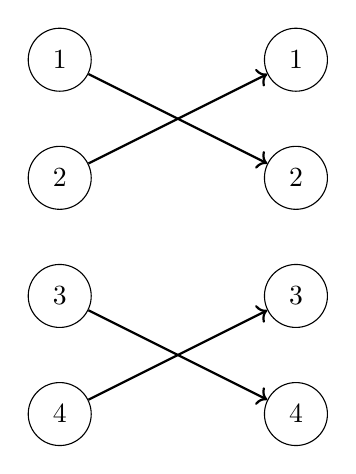
\begin{tikzpicture}[scale=1]
  % 定义集合A的元素
  \foreach \i in {1,2,3,4} {
    \node[draw, circle, minimum size=0.8cm] (a\i) at (0, 2.5 - \i * 1.5) {\i};
    \node[draw, circle, minimum size=0.8cm] (b\i) at (3, 2.5 - \i * 1.5) {\i};
  }
  
  % 绘制映射关系
  \draw[->, thick] (a1) -- (b2);
  \draw[->, thick] (a2) -- (b1);
  \draw[->, thick] (a3) -- (b4);
  \draw[->, thick] (a4) -- (b3);
\end{tikzpicture}

\item 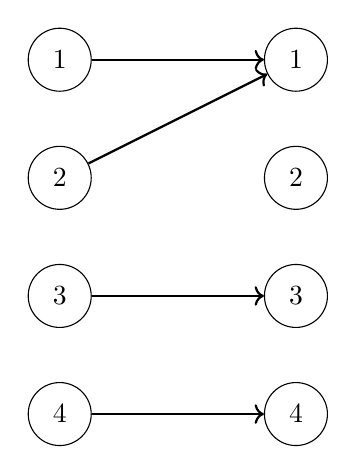
\begin{tikzpicture}[scale=1]
  % 定义集合A的元素
  \foreach \i in {1,2,3,4} {
    \node[draw, circle, minimum size=0.8cm] (a\i) at (0, 2.5 - \i * 1.5) {\i};
    \node[draw, circle, minimum size=0.8cm] (b\i) at (3, 2.5 - \i * 1.5) {\i};
  }
  
  % 绘制映射关系（非单射，例如元素1和2都映射到元素1）
  \draw[->, thick] (a1) -- (b1);
  \draw[->, thick] (a2) -- (b1);
  \draw[->, thick] (a3) -- (b3);
  \draw[->, thick] (a4) -- (b4);
\end{tikzpicture}
\item $4$ 个元素每个都有 $4$ 种选择，共计 $4^4 = 256$ 种。
\end{enumerate}
  \end{solution}

  
\item 设 \(\mathbb{N}\) 表示自然数集。绘制由 \(n \mapsto  {n}^{2}\) 定义的映射 \(\mathbb{N} \rightarrow  \mathbb{N}\) 的部分图像。这是单射吗？

  \begin{solution}
\begin{tikzpicture}[scale=0.8]
    % 绘制坐标轴
    \draw[->] (0,0) -- (8,0) node[right] {\(n\)};
    \draw[->] (0,0) -- (0,8) node[above] {\(n^2\)};

    % 添加刻度
    \foreach \x in {0,1,...,7}
        \draw (\x,0) -- (\x,-0.1) node[below] {\x};
    \foreach \y in {0,1,...,7}
        \draw (0,\y) -- (-0.1,\y) node[left] {\y};

    % 绘制映射点
    \foreach \n in {0,1,2,3}
        \fill (\n,{\n*\n}) circle (2pt);

    % 添加映射箭头
    \foreach \n in {0,1,2,3}
        \draw[->,shorten >=2pt,shorten <=2pt] (\n,0) -- (\n,{\n*\n});

    % 添加标签
    \node at (4,6) [above] {\(n \mapsto n^2\)};
\end{tikzpicture}
    
    是单射。
  \end{solution}
  
\item 若已知某映射是单射，其图像的行有何特征？

  \begin{solution}
每行至多有一个元素。    
  \end{solution}
  
\end{enumerate}


\section*{满射}

\begin{enumerate}
  \setcounter{enumi}{8}
\item 绘制下列映射 \(\mathbb{Q} \rightarrow  \mathbb{Q}\) 的示意图:
\begin{enumerate}
\item \(\alpha  : x \mapsto  {2}^{x}\) 
\item \(\beta  : x \mapsto  x + 1\) 。
\end{enumerate}
对于任意 \(y \in \mathbb{Q}\) ，是否总能找到 \(x \in \mathbb{Q}\) 使得 \(\alpha  : x \mapsto  y\) 成立？

对于任意实数 \(y \in \mathbb{Q}\) ，是否总能找到 \(x\in \mathbb{Q}\) 使得 \(\beta  : x \mapsto  y\) 成立？

\begin{solution}
\begin{tikzpicture}[scale=1.2, >=Stealth]

% 第一个图：alpha: x ↦ 2^x
\begin{scope}[xshift=0cm]
    % 坐标轴
    \draw[->] (-2.5,0) -- (2.5,0) node[right] {$x$};
    \draw[->] (0,-0.5) -- (0,4.5) node[above] {$y$};
    
    % 函数图像：2^x
    \draw[domain=-2:2, smooth, variable=\x, thick, blue] plot ({\x}, {2^\x});
    
    % 标注
    \node[below left] at (0,0) {$0$};
    \node[above] at (0,5.5) {$\alpha(x)=2^x$};
    \node[below] at (0,-0.5) {};
\end{scope}

% 第二个图：beta: x ↦ x + 1
\begin{scope}[xshift=7cm]
    % 坐标轴
    \draw[->] (-2.5,0) -- (2.5,0) node[right] {$x$};
    \draw[->] (0,-1.5) -- (0,3.5) node[above] {$y$};
    
    % 函数图像：x + 1
    \draw[domain=-2.5:2.5, thick, red] plot (\x, {\x + 1});
    
    % 标注
    \node[below left] at (0,0) {$0$};
    \node[above] at (0,4.5) {$\beta(x)=x+1$};
\end{scope}

\end{tikzpicture}

  
  不能；可以。
\end{solution}



由此差异可称 \(\beta\) 为满射，而 \(\alpha\) 不是满射。

\item  设 \(A = \{ 1,2,3,4\}\) 。展示一个映射 \(A \rightarrow  A\) 的图像，使得其分别满足
\begin{enumerate}
\item 该映射是满射。
\item 该映射不是满射。
\end{enumerate}

\begin{solution}
  \begin{enumerate}
  \item



\begin{tikzpicture}[
    dom/.style={circle, draw, fill=blue!20, minimum size=8mm}, % 修改了样式名称
    ran/.style={circle, draw, fill=red!20, minimum size=8mm},  % 修改了样式名称
    arrow/.style={->, >=Stealth, thick}
]

% 定义域节点 (左侧)
\node[dom] (d1) at (0,3) {1};
\node[dom] (d2) at (0,2) {2};
\node[dom] (d3) at (0,1) {3};
\node[dom] (d4) at (0,0) {4};

% 值域节点 (右侧)
\node[ran] (r1) at (3,3) {1};
\node[ran] (r2) at (3,2) {2};
\node[ran] (r3) at (3,1) {3};
\node[ran] (r4) at (3,0) {4};

% 映射关系 (满射)
\draw[arrow] (d1) -- (r2);
\draw[arrow] (d2) -- (r3);
\draw[arrow] (d3) -- (r4);
\draw[arrow] (d4) -- (r1);

% 标签
\node at (0,4) {定义域};
\node at (3,4) {值域};
\node[align=center] at (1.5,4) {满射映射 \\ $f(1)=2,\ f(2)=3,\ f(3)=4,\ f(4)=1$};
\end{tikzpicture}


\item 
\begin{tikzpicture}[
    dom/.style={circle, draw, fill=blue!20, minimum size=8mm}, % 修改了样式名称
    ran/.style={circle, draw, fill=red!20, minimum size=8mm},  % 修改了样式名称
    arrow/.style={->, >=Stealth, thick}
]

% 定义域节点 (左侧)
\node[dom] (d1) at (0,3) {1};
\node[dom] (d2) at (0,2) {2};
\node[dom] (d3) at (0,1) {3};
\node[dom] (d4) at (0,0) {4};

% 值域节点 (右侧)
\node[ran] (r1) at (3,3) {1};
\node[ran] (r2) at (3,2) {2};
\node[ran] (r3) at (3,1) {3};
\node[ran] (r4) at (3,0) {4};

% 映射关系 (非满射)
\draw[arrow] (d1) -- (r1);
\draw[arrow] (d2) -- (r1);
\draw[arrow] (d3) -- (r1);
\draw[arrow] (d4) -- (r1);

% 标签
\node at (0,4) {定义域};
\node at (3,4) {值域};
\node[align=center] at (1.5,4) {非满射映射 \\ $f(x)=1$ 对所有 $x \in A$};
\end{tikzpicture}
  \end{enumerate}
\end{solution}


\item  绘制由以下定义映射 \(\mathbb{N} \rightarrow  \mathbb{N}\) 的部分图像:
  $$
n \mapsto
\begin{cases}
  \frac{n}{2} & n \text{为偶数} \\
  \frac{n+1}{2} & n \text{为奇数}
\end{cases}
  $$
  这是单射吗？这是一个满射吗？

  \begin{solution}
    \begin{tikzpicture}[scale=0.8]
  % 绘制坐标轴
  \draw[->] (-0.5,0) -- (11,0) node[right] {$n$};
  \draw[->] (0,-0.5) -- (0,6) node[above] {$f(n)$};
  
  % 绘制网格
  \foreach \x in {0,1,...,10} {
    \draw[gray,very thin] (\x,-0.1) -- (\x,5.5);
  }
  \foreach \y in {0,1,...,5} {
    \draw[gray,very thin] (-0.1,\y) -- (10.5,\y);
  }
  
  % 标记坐标轴刻度
  \foreach \x in {0,1,...,10} {
    \node[below] at (\x,0) {\x};
  }
  \foreach \y in {0,1,...,5} {
    \node[left] at (0,\y) {\y};
  }
  
  % 绘制映射点
  % 偶数点：n/2
  \foreach \x in {0,2,4,6,8,10} {
    \pgfmathsetmacro{\y}{\x/2}
    \fill[blue] (\x,\y) circle (2pt);
  }
  
  % 奇数点：(n+1)/2
  \foreach \x in {1,3,5,7,9} {
    \pgfmathsetmacro{\y}{(\x+1)/2}
    \fill[red] (\x,\y) circle (2pt);
  }
  
  % 添加一些标记
  \node[blue] at (10,0) [above right] {偶数: $f(n)=n/2$};
  \node[red] at (10,0) [right] {奇数: $f(n)=(n+1)/2$};
  
  % 绘制连接线（可选，显示映射关系）
  \draw[dashed,gray] (0,0) -- (2,1);
  \draw[dashed,gray] (1,1) -- (2,1);
  \draw[dashed,gray] (2,1) -- (4,2);
  \draw[dashed,gray] (3,2) -- (4,2);
  \draw[dashed,gray] (4,2) -- (6,3);
  \draw[dashed,gray] (5,3) -- (6,3);
  \draw[dashed,gray] (6,3) -- (8,4);
  \draw[dashed,gray] (7,4) -- (8,4);
  \draw[dashed,gray] (8,4) -- (10,5);
  \draw[dashed,gray] (9,5) -- (10,5);
  
  % 添加标题
  \node[above] at (5,5.5) {映射 $f: \mathbb{N} \to \mathbb{N}$ 的部分图像};
\end{tikzpicture}
是满射，不是单射。
  \end{solution}
  

\item  关于满射映射图像的行，我们能得出什么结论？

  \begin{solution}
    每行至少有一个元素。
  \end{solution}
  
\item  设 \(A = \{ 1,2,3,4\}\) 。
\begin{enumerate}
\item 能否构造一个单射但不满射的映射 \(A \rightarrow  A\) ？
\item 能否构造一个满射但不单射的映射 \(A \rightarrow  A\) ？
\end{enumerate}

\begin{solution}
  不能。不能。
\end{solution}


\item 能否构造一个单射但不满射的映射 \(\mathbb{N} \rightarrow  \mathbb{N}\) ？能否构造一个满射但不单射的映射 \(\mathbb{N} \rightarrow  \mathbb{N}\) ？
  \begin{solution}
    单射不满射：$n \mapsto n^2$

    满射不单射：$n \mapsto \left\lfloor \frac{n}{2} \right\rfloor$
  \end{solution}

\item  推测任意集合 \(A\) 所需满足的条件，使得每个单射映射 \(A \rightarrow  A\) 都必须是满射的，且每个满射映射 \(A \rightarrow  A\) 都必须是单射的。借助问题8和问题12证明你的猜想。

  \begin{solution}
    命题成立当且仅当 $A$ 是有限集。

    证明：
    \begin{itemize}
    \item 单射$\Rightarrow$满射：设 $f: A\to A$ 为单射，则 $\left| f(A) \right| = \left| A \right|$。又 $f(A)\subset A$ 且二者皆为有限集，这唯有 $f(A) = A$，即 $f$ 是满射。
    \item 满射 $\Rightarrow$ 单射：反设 $f : A\to A$ 是满射但不是单射，则 $\left| f(A) \right| < \left| A \right|$。然而满射要求 $\left| f(A) \right| = \left| A \right|$，矛盾！
    \end{itemize}
  \end{solution}

  
既是单射又是满射的映射称为双射。在定义域和陪域相同的有限集映射中，单射、满射和双射实际上无法区分。

\item  举例说明映射 \(\mathbb{Q} \rightarrow  \mathbb{Q}\) 的以下情形:
\begin{enumerate}
\item 单射且满射，

\item  单射但非满射，

\item  满射但非单射，

\item  既非单射也非满射。
\end{enumerate}

\begin{solution}
  \begin{enumerate}
  \item $x\mapsto x$
  \item $x\mapsto 2^x$
  \item $x\mapsto x^3 - x$
  \item $x\mapsto x^2$
  \end{enumerate}
\end{solution}

 
\item 若存在一个单射但不满射的映射 \(A \rightarrow  A\) ，关于集合 \(A\) 能得出什么结论？
  \begin{solution}
    $A$ 不是有限集。
  \end{solution}
\end{enumerate}

\section*{映射的复合}

\begin{enumerate}
  \setcounter{enumi}{17}
\item 若 \(\alpha\) 和 \(\beta\) 是由以下定义确定的映射 \(\mathbb{Q} \rightarrow  \mathbb{Q}\)

\[\alpha  : x \mapsto  {2x}, \quad \beta  : x \mapsto  x + 1\]

那么我们定义 \({x\beta } : x \mapsto  {2x} + 1\) 。

\[
x \mapsto  {2x} \mapsto  {2x} + 1
\]

我们将其记为 \(\left( x\right) {\alpha \beta } = \left( {2x}\right) \beta  = {2x} + 1\) 。

根据类似定义确定 \(\left( x\right) {\beta \alpha}\) 。

\begin{solution}
  $2x + 2$
\end{solution}

\item  若 \(\alpha  : A \rightarrow  B\) 和 \(\beta  : B \rightarrow  C\) 是映射，请通过确定 \(\left( x\right) {\alpha \beta }\) 给出 \({\alpha \beta } : A \rightarrow  C\) 的形式化定义。

  \begin{solution}
    给定 $x \in A$，定义 $(x)\alpha\beta = \left( (x)\alpha \right)\beta$ 
  \end{solution}

映射 \({\alpha \beta }\) 称为映射 \(\alpha\) 与 \(\beta\) 的复合。

\item 已知 $\alpha, \beta$ 的示意图如下，试绘制 $\alpha\beta$ 的示意图。

  \begin{center}
     \includegraphics[width = 0.4\linewidth]{images/fig-5.png}
   \end{center}

   \begin{solution}
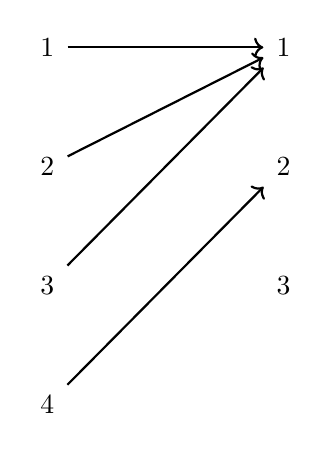
\begin{tikzpicture}[
    node distance=1cm,
    every node/.style={minimum size=0.5cm},
    arrow/.style={->, thick}
]

% 左侧节点
\node (a1) at (0,0) {1};
\node (a2) [below=of a1] {2};
\node (a3) [below=of a2] {3};
\node (a4) [below=of a3] {4};

% 右侧节点
\node (b1) at (3,0) {1};
\node (b2) [below=of b1] {2};
\node (b3) [below=of b2] {3};

% 绘制箭头
\draw[arrow] (a1) -- (b1);
\draw[arrow] (a2) -- (b1);
\draw[arrow] (a3) -- (b1);
\draw[arrow] (a4) -- (b2);

\end{tikzpicture}

   \end{solution}

 \item   “\(\alpha  : A \rightarrow  B\) 是单射”，试给出其形式定义。

   \begin{solution}
     $\forall x, y \in A, (x)\alpha = (y)\alpha \Rightarrow b_1 = b_2$
   \end{solution}

 \item  若 \(\alpha  : A \rightarrow  B\) 和 \(\beta  : B \rightarrow  C\) 都是单射，能推出 \({\alpha \beta } : A \rightarrow  C\) 的什么性质？

   \begin{solution}
     $\alpha\beta$ 犹为单射。

     证明：$\forall x,y \in A, (x)\alpha\beta = (y)\alpha\beta \Rightarrow (x)\alpha = (y)\alpha \Rightarrow x = y $
   \end{solution}

\item  设 \(A = \{ 1,2,3\}\) 和 \(B = \{ 1,2,3,4\}\) ，并令 \(\alpha  : A \rightarrow  B\) 为单射。

能否构造满足以下条件的映射 \(\beta  : B \rightarrow  A\) :

\begin{enumerate}
\item \({\beta \alpha }\) 是恒等映射 \(B \rightarrow  B\) ，
\item  \({\alpha \beta }\) 是恒等映射 \(A \rightarrow  A\) 
\end{enumerate}

\begin{solution}
  \begin{enumerate}
  \item 不能，因为 $\left| (A)\alpha \right| < \left| A \right|$
  \item 可以。对于 $(A)\alpha$ 中的元素$(x)\alpha$，只需令 $ \left( (x)\alpha \right)\beta = x$；对于剩余的一个元素，随意指定其象即可。
  \end{enumerate}
\end{solution}
\end{enumerate}


\section*{逆映射}
\begin{enumerate}
  \setcounter{enumi}{23}
\item 设 \(A\) 和 \(B\) 为任意集合，且 \(\alpha  : A \rightarrow  B\) 为单射。请说明如何定义 \(\beta  : B \rightarrow  A\) 使得 \({\alpha \beta }\) 成为 \(A\) 上的恒等映射。

  \begin{solution}
    对于 $(A)\alpha$ 中的元素$(x)\alpha$，只需令 $ \left( (x)\alpha \right)\beta = x$；对于剩余的元素，随意指定其象即可。
  \end{solution}

  此时映射 \(\beta\) 称为 \(\alpha\) 的右逆。因此单射具有右逆。
\item  “\(\alpha  : A \rightarrow  B\) 是满射”，试给出其形式定义。

  \begin{solution}
    $\forall b \in B, \exists a \in A \text{ s.t. }  (a)\alpha = b$
  \end{solution}

  
\item 若 \(\alpha  : A \rightarrow  B\) 和 \(\beta  : B \rightarrow  C\) 都是满射，复合映射 \({\alpha \beta } : A \rightarrow  C\) 具有什么性质？

  \begin{solution}
    $\alpha\beta$ 犹为满射。

    证明：给定 $c \in C, \exists b \in B \text{ s.t. }  c = (b)\beta, \exists a \in A \text{ s.t. }  b= (a)\alpha \Rightarrow c = (a)\alpha\beta$
  \end{solution}

  
\item 设 \(A = \{ 1,2,3,4\}\) 和 \(B = \{ 1,2,3\}\) ，且 \(\alpha  : A \rightarrow  B\) 为满射。
\begin{enumerate}
\item 能否构造映射 \(\beta  : B \rightarrow  A\) 使得 \({\alpha \beta }\) 成为 \(A\) 上的恒等映射？
\item 能否构造映射 \(\beta  : B \rightarrow  A\) 使得 \({\beta \alpha } : B \rightarrow  B\) 成为 \(B\) 上的恒等映射？
\end{enumerate}

\begin{solution}
\begin{enumerate}
\item 不能。
\item 可以。因 $\alpha$ 是满射，$\forall b \in B, \exists a \in A \text{ s.t. }  b = (a)\alpha$。只需指定 $(b)\beta = a$ 即可：$(b)\beta\alpha = (a)\alpha = b$。
\end{enumerate}
\end{solution}

\item 设 \(A\) 和 \(B\) 为任意集合，其中 \(\alpha  : A \rightarrow  B\) 是满射。证明如何定义映射 \(\beta  : B \rightarrow  A\) 使得 \({\beta \alpha }\) 成为 \(B\) 上的恒等映射？

  \begin{solution}
    因 $\alpha$ 是满射，$\forall b \in B, \exists a \in A \text{ s.t. }  b = (a)\alpha$。只需指定 $(b)\beta = a$ 即可：$(b)\beta\alpha = (a)\alpha = b$。
  \end{solution}
  

  此时映射 \(\beta\) 称为 \(\alpha\) 的左逆。故满射必存在左逆。
\item 设 \(A = \{ 1,2,3\}\) 。列出所有双射 \(A \rightarrow  A\) ，即 \(A\) 的所有排列。求每个双射的左逆和右逆。

  \begin{solution}
    双射的左逆与右逆相等。

    以下映射的逆就是自身：
    \begin{itemize}
    \item $1\mapsto 1, 2\mapsto 2, 3\mapsto 3$
    \item $1\mapsto 2, 2\mapsto 1, 3\mapsto 3$
    \item $1\mapsto3, 2\mapsto 2, 3\mapsto 1$
    \item $1\mapsto1, 2\mapsto 3, 3\mapsto2$
    \end{itemize}

    以下两映射互为逆
    \begin{itemize}
    \item $1\mapsto2, 2\mapsto 3, 3\mapsto 1$
    \item $1\mapsto 3, 2\mapsto 1, 3\mapsto 2$
    \end{itemize}
  \end{solution}
  
\item 对任意双射 \(\alpha  : A \rightarrow  B\) ，定义双射 \(\beta  : B \rightarrow  A\) 使得 \({\alpha \beta }\) 为恒等映射 \(I_A : A \rightarrow  A\) 且 \({\beta \alpha }\) 为恒等映射 \(I_B : B \rightarrow  B\) 。

  证明 \({\alpha \beta } = I_A : A \rightarrow  A\) 或 \({\beta \alpha } = I_B : B \rightarrow  B\) 能唯一确定 \(\beta\) 。

  \begin{proof}
    \begin{enumerate}
    \item 已知 $\alpha\beta = I_A$。$\forall b \in A$，我们需唯一地确定 $(b)\beta$。

      因 $\alpha$ 是满射，$\exists a \in A \text{ s.t. }  b = (a)\alpha$。

      两边作用 $\beta$ 得 $(b)\beta = (a)\alpha\beta$。然而 $\alpha\beta = I_A$，这便要求 $(a)\alpha\beta = a$。代回得 $(b)\beta = a$。

      设 $a' \in A$ 同样满足 $b = (a')\alpha$（于是 $(b)\beta = a'$） ，因 $\alpha$ 是单射 $(a)\alpha = (a')\alpha \Rightarrow a = a'$。于是 $(b)\beta = a$ 的取值是唯一的。
    \item 已知 $\beta\alpha = I_B$。$\forall b \in B$，我们需要唯一地确定 $(b)\beta$。

      由条件 $(b)\beta \alpha = b$。因 $\alpha$ 是满射，$\exists a \in A \text{ s.t. }  b = (a)\alpha$，代回得 $\left( (b) \beta \right) \alpha = (a)\alpha$。又因 $\alpha$ 是单射（可右消去），$(b)\beta = a$。
    \end{enumerate}
  \end{proof}

因此双射具有双侧逆。
\end{enumerate}


\section*{封闭性}

\begin{enumerate}
\setcounter{enumi}{30}
\item 若 \(\alpha\) 和 \(\beta\) 都是双射 \(A \rightarrow  A\) ，则 \({\alpha \beta } : A \rightarrow  A\) 具有什么性质？
\end{enumerate}

\begin{solution}
  $\alpha\beta$ 犹为双射。

  证明：$\alpha,\beta$ 均为单射 $\Rightarrow \alpha\beta$ 为单射。$\alpha,\beta$ 均为满射 $\Rightarrow \alpha\beta$ 为满射。综上得证。
\end{solution}


\section*{结合律}

\begin{enumerate}
  \setcounter{enumi}{31}
\item 设 \(\alpha  : A \rightarrow  B,\beta  : B \rightarrow  C\) 和 \(\gamma  : C \rightarrow  D\) 为映射。利用问题19的定义证明:对于 \(A\) 的每个元素 \(x\) ，都有

\[\left( x\right) \left\lbrack  {\left( {\alpha \beta }\right) \gamma }\right\rbrack   = \left( x\right) \left\lbrack  {\alpha \left( {\beta \gamma }\right) }\right\rbrack  ,\]

\begin{proof}
  两者都等于 $(((x)\alpha)\beta)\gamma$
\end{proof}

由此，两个映射 \(A \rightarrow  D,\left( {\alpha \beta }\right) \gamma\) 与 \(\alpha \left( {\beta \gamma }\right)\) 不可区分。

定理 \(\left( {\alpha \beta }\right) \gamma  = \alpha \left( {\beta \gamma }\right)\) 称为映射复合运算的结合律。

\item  运用结合律证明:对于四个映射 \(\alpha  : A \rightarrow  B\) 、 \(\beta  : B \rightarrow  C,\gamma  : C \rightarrow  D,\delta  : D \rightarrow  E\) ，有 \(\alpha \left\lbrack  {\beta \left( {\gamma \delta }\right) }\right\rbrack   = \left\lbrack  {\left( {\alpha \beta }\right) \gamma }\right\rbrack  \delta\) 。

  \begin{solution}
    
\[
\alpha\left[ \beta \left( \gamma \delta \right) \right] = \alpha\left[ \left( \beta \gamma \right) \delta \right] = \left[ \alpha \left( \beta \gamma \right) \right] \delta=\left[ \left( \alpha \beta \right) \gamma \right] \delta.
\]

  \end{solution}
  
  \section*{对称群}

\item  设 \(\mathfrak{S}\) 为所有双射 \(A \rightarrow  A\) 的集合。证明下列每个命题。
\begin{enumerate}
\item 【封闭性】若 \(\alpha\) 和 \(\beta\) 属于 \(\mathfrak{S}\) ，则 \({\alpha \beta }\) 也属于 \(\mathfrak{S}\) 。

\item 【结合性】若 \(\alpha ,\beta\) 和 \(\gamma\) 属于 \(\mathfrak{S}\) ，则 \(\alpha \left( {\beta \gamma }\right)  = \left( {\alpha \beta }\right) \gamma\) 。

\item  【单位元】由 \(I : x \mapsto  x\) 定义的 \(I : A \rightarrow  A\) (对所有 \(A\) 中的 \(x\) )属于 \(\mathfrak{S}\) 。对所有 \(\mathfrak{S}\) 中的 \(\alpha\) 有 \({I\alpha } = {\alpha I} = \alpha\) 。

\item  【逆元】对于 \(\mathfrak{S}\) 中的每个 \(\alpha\) ，存在 \(\mathfrak{S}\) 中的 \(\beta\) 使得 \({\alpha \beta } = {\beta \alpha } = I\) 。
\end{enumerate}
这四个定理可总结为:集合到自身的双射在复合运算下构成群。此情形下的群称为 \(A\) 上的对称群，记作 \({\mathfrak{S}}_{A}\) 。

\begin{proof}
  \begin{enumerate}
  \item 见问题 31
  \item 见问题 32
  \item 构造 $\forall a \in A, (a)I = a$
  \item 见问题 30
  \end{enumerate}
\end{proof}
\end{enumerate}

}




%\end{multicols} % End the two-column environment


% Use \newpage or \clearpage to start a new page if needed.
% \clearpage


% Label this page as 'LastPage' for the footer reference
\label{LastPage}
\end{document}
% =============================================================================
% END OF DOCUMENT
% =============================================================================

%%% Local Variables:
%%% mode: latex
%%% TeX-master: t
%%% End:
